\problemname{Armstöd}

Petitess-organisationen (PO) har möte och de $N$ medlemmarna sitter på inåtvända stolar i en ring. Mellan varje par av stolar finns ett armstöd som högst en av personerna kan använda. Varje person har en preferens i form av vilken eller vilka armar hen vill placera på armstöden:
\begin{list}
\item V: vänster arm
\item H: höger arm
\item A: antingen vänster eller höger arm
\item B: båda armarna
\item I: ingen arm
\end{list}

Skriv ett program som beräknar hur många av personerna som maximalt kan bli nöjda.

\begin{figure}[h] 
\begin{center}
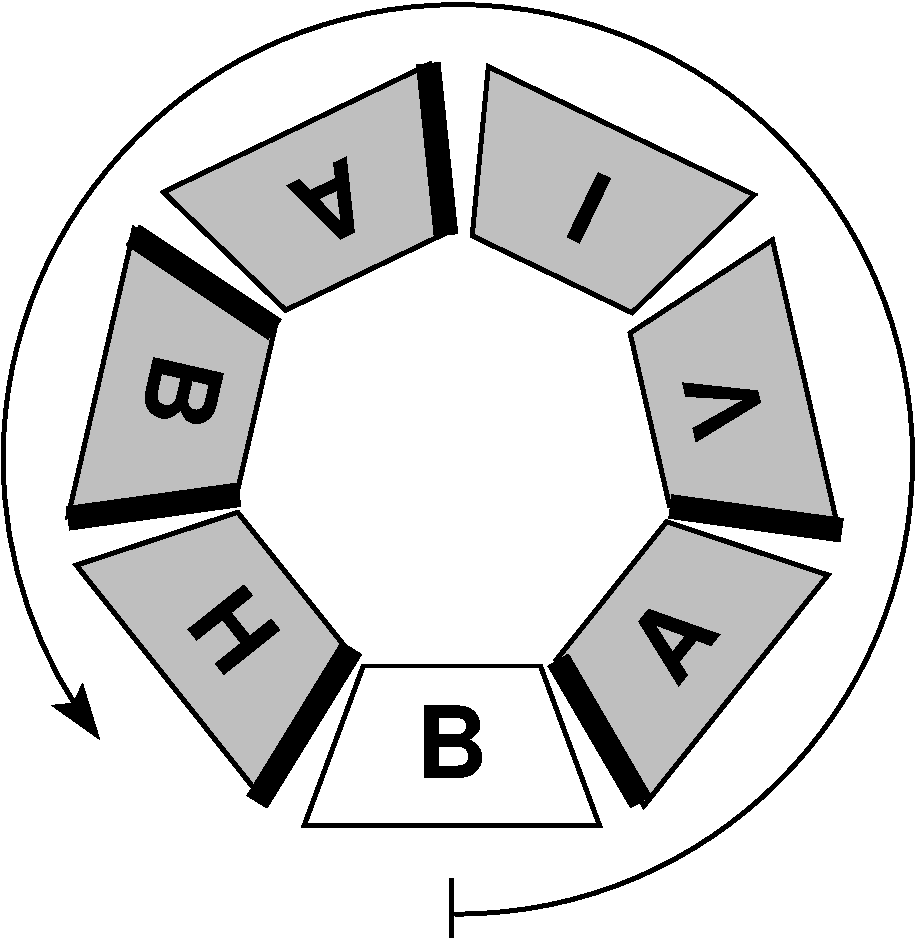
\includegraphics[width=8cm]{armstodbild.pdf}
\caption{Lösningen på det andra körningsexemplet. De tjocka linjerna markerar armar på armstöden. De skuggade polygonerna motsvarar de sex personer som har fått sina preferenser uppfyllda. Pilen markerar var den givna indatasträngen börjar och slutar.}
\end{center} 
\end{figure}

\section*{Indata}
Programmet ska läsa in ett heltal $N$, antal personer i ringen. Därefter en rad med $N$ bokstäver, vardera \tt{V}, \tt{H}, \tt{A}, \tt{B} eller \tt{I}, preferenserna för personerna i ringen, givna moturs i den ordning de sitter.

\section*{Utdata}
Progrmmet ska skriva ut ett tal: det maximala antalet personer som kan få sin preferens uppfylld.

\section*{Poängsättning}

För testfall värda 
\begin{tabular}{llll}
$1$ poäng & gäller att &N=5$ & och första bokstaven är I. \\
$2$ poäng &  & $6\le N\le 15$ &, vilka bokstäver som helst.\\
$1$ poäng &  & $25\le N\le 30$ & och första bokstaven är I. \\
$1$ poäng &  & $25\le N\le 30$ &, vilka bokstäver som helst. \\
\end{tabular}                          
